\documentclass{article}

\usepackage[sort&compress,numbers]{natbib}
\usepackage{multicol}
\usepackage{etoolbox}
\usepackage{subfig}
\usepackage{tikz}
    \usetikzlibrary{colorbrewer}
    \usetikzlibrary{patterns}
    \usetikzlibrary{spy}
\usepackage{float}
\usepackage[framemethod=default]{mdframed}
\usepackage[a4paper, margin=1in]{geometry}
\usepackage{enumitem}
\usepackage{xcolor}
\usepackage{graphicx}
\usepackage{pgfplots}
    \usepgfplotslibrary{colorbrewer}

\setlist{noitemsep, topsep=0pt}

\newcommand{\TODO}[1]{\noindent{\color{red}\textbf{[TODO] #1}}}
\newcommand{\floor}[1]{\left\lfloor #1 \right\rfloor}
\newcommand{\ceil}[1]{\left\lceil #1 \right\rceil}
\newrobustcmd*{\square}[1]{\tikz{\filldraw[draw=#1,fill=#1] (0,0) rectangle (0.22cm,0.22cm);}}

\title{Improving Performance in Structured GPGPU Workloads via Specialized Thread Schedules}
\author{Naraendra Prasetya}
\date{2021}

\begin{document}

\maketitle

\section{Introduction}    
High performance GPU computing has become very accessible via high level frameworks.
These frameworks provide a limited set of operators, such as stencil, permute, fold, scan, which can manipulate data on a GPU \cite{chakravarty2011accelerating}.
However, in most cases the compiled assembly has inefficient memory accesses with lower cache hit rates and uncoalesced accesses.
Threads can be scheduled in such a way to minimize these inefficiencies.
With a smarter scheduler, programs can achieve better cache and memory utilization \cite{nugteren2014study}.
We propose several specialized thread schedules to improve performance by leveraging the structure of memory accesses in the high level GPGPU framework Accelerate.

\subsection{GPU Architecture}
Massive parallel workloads are executed on numerous cores clustered in streaming multiprocessors (SMs).
The memory is structured in a multi-level hierarchy containing a L1 cache for each SM, a shared L2 cache for all SMs and multiple banks of DRAM \cite{nvidia2017volta,nvidia2020ampere}.

Memory can become a significant bottleneck due to the large amount of threads running concurrently.
Caches can alleviate this but is limited in size, and given a large enough problem can cause cache trashing -- the premature eviction of cache lines before any significant reuse \cite{dai2016model}.

Data shared between threads through the cache can happen read-after-write (RAW) or read-after-read (RAR).
RAW has data dependency among tasks, for example in scan operations.
RAR has no data dependency and can be executed in any order \cite{tripathy2021paver}.

The L1 cache in older Nvidia GPU architectures (Maxwell, Pascal) uses the least recently used (LRU) eviction policy, new architectures (Turing, Volta) uses a non-LRU eviction policy \cite{jia2019dissecting, jia2018dissecting,mei2016dissecting}.
\citet{jia2019dissecting} has shown that in Turing and Volta GPU's, the P-chase benchmark presented by \citet{mei2016dissecting} fails to detect the full L1 cache.
This is due to the new L1 eviction policy introduced with Volta, where cache lines can be assigned a priority \cite{jia2019dissecting,nvidia2021cudadocs}.

A program instructs what a single thread most do, given certain runtime and constant variables.
Executing a program spawns multiple threads, each with their own thread id and corresponding block id.
These threads are grouped into cooperative thread arrays (CTA), sometimes also called a thread block.
A CTA gets executed in SIMT in groups called warps which typically contain 32 threads.
There is a maximum number of threads that can fit a CTA, so we often need multiple.

% Cache hitrate
% Memory coalescing 

\subsection{Accelerate}
Accelerate is an embedded purely functional array language in Haskell \cite{chakravarty2011accelerating}.
Accelerate has a frontend containing the embedded language, and the backend which handles code generation and execution.
Programs can be defined within the embedded language, where they may also be optimized via fusion.
Further hardware specific optimization is handled on the various backends.
There are two backends provided: one that targets multicore CPUs \texttt{accelerate-llvm-native} and one that targets Nvidia GPUs \texttt{accelerate-llvm-ptx}.
The PTX backend implements a series of CUDA skeletons which implement a series of primitive operations such as stencils, generate, permute, and scan.
These skeletons define how a program should be compiled and is the part where a custom thread scheduler can be implemented.
Further customizations to the scheduler can be done on the executing side of the backend as it controls how kernels are launched.

\section{Related Work}

\subsection{Cache Locality}
\citet{meyer2003algorithms} describes two principles of locality:
\begin{itemize}
    \item \textbf{Spatial locality:} Accessing a block of data should contain as much useful data as possible.
    \item \textbf{Temporal locality:} Once a data block is cached, as much work with it should be done before it is evicted.
\end{itemize}
Furthermore, if a program is memory bound, we want to increase either or both types of locality depending on the application and hardware.

However, to generate cache-aware programs, we need to know when what gets accessed.
\citet{koo2015revealing} proposes a categorization between deterministic and non-deterministic loads.
A memory access is deterministic when the referenced address is generated from parameterized data such as CTA ids, thread ids, and constant parameters.
This classification can be done via backward data flow analysis. The structure of these deterministic loads can be exploited to generate better schedules for threads.
Deterministic loads are more likely to have coalesced memory access patterns. 
Non-deterministic loads will generate more memory requests due to uncoalesced memory accesses.
\citet{koo2015revealing} concludes that a smart CTA scheduler can improve performance.

\subsection{CTA Clustering}
Because CTAs are assigned to SMs in a round-robin fashion, nearby CTAs may not be able to exploit the L1 cache as they can be assigned to different SMs.
We call this sharing between CTAs inter-CTA locality.
Not every program has inter-CTA locality, for example: incrementing every element by a fixed amount.
Inter-CTA locality can be categorized into:
\begin{itemize}
    \item Algorithm related locality present promising opportunities for inter-CTA reuse.
    \item Cache-line related locality result from non-aligned memory accesses or coalesced.
    \item Locality stemming from irregular data structures (pointers) often happens by accident and is thus difficult to account for.
    \item Write related applications may suffer when multiple CTAs write to the same cache line causing an eviction in the L1 cache.
    \item Streaming applications are coalesced and aligned.
\end{itemize}
\citet{li2017locality} proposes a clustering algorithm for CTAs.
For algorithmic locality, the partitioning is based on a dependency analysis on the array references.
The CTAs are then remapped according to a set of patterns.
These are executed normally or via an agent based system \cite{li2017locality}.
\TODO{Relate to proposal}

\subsection{Locality Graph-Based Scheduling}
\citet{tripathy2021paver} presented a priority aware vertex scheduler (PAVER) for read-after-read programs which expands on the previous work.
PAVER does not work with read-after-write programs, as those might result in a deadlock with the implemented scheduler.
It derives a locality graph from PTX code which can be partitioned to maximize data sharing between SMs.
The partitioned work is stored as queue of thread block groups.
Each SM runs a dedicated worker which gets a thread block group from the global queue and then goes through the thread blocks within the group.
If an SM has no more work, it steals work from other SMs by taking from the tail of the thread block group.

\subsection{Stencil Computations}
Stencil operations update an N-dimensional array according to a fixed pattern surrounding the updated element (fig. \ref{fig:stencil_access_pattern}).

\begin{figure}[H]
    \centering
    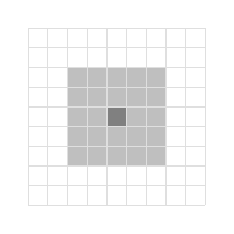
\begin{tikzpicture}[scale=0.25]
        \fill[gray!50] (2, 2) rectangle +(5, 5);
        \fill[gray!100] (4, 4) rectangle +(1, 1);
        \draw[step=1,gray!25] (0, 0) grid (9, 9);
    \end{tikzpicture}
    \caption{
        The access pattern for a 5x5 stencil operation on a single element \square{gray!100} that accesses \square{gray!50}.
    }
    \label{fig:stencil_access_pattern}
\end{figure}

Improving the performance of stencil computations have been researched extensively.
\citet{kamil2006implicit} presented optimizations targeting temporal cache reuse across multiple stencil sweeps via time skewing.
\citet{zhao2019exploiting} presented a vectorization approach and improvements regarding instruction cache hits.
However, none of the presented optimizations try to tackle temporal locality within a stencil sweep.
\TODO{Expand on this}

\subsection{Matrix Computations}
\label{sec:matrix_intro}
Matrix multiplication take two 2D input matrices to produce a new output matrix $C = AB$ and is defined as
\[
    c_{ij} = \sum^n_k{a_{ik}b_{kj}}
\]
In terms of memory accesses, for each element, a row and a column needs to be accessed (fig. \ref{fig:matmult_access_pattern}).

\begin{figure}[h]
    \centering
    \subfloat[Different arrays stacked.]{
        \centering
        \makebox[0.4\columnwidth][c]{
            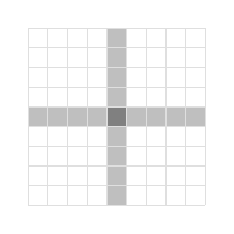
\begin{tikzpicture}[scale=0.25]
                \fill[gray!50]  (0, 4) rectangle +(9, 1);
                \fill[gray!50]  (4, 0) rectangle +(1, 9);
                \fill[gray!100] (4, 4) rectangle +(1, 1);
                \draw[step=1,gray!25] (0, 0) grid (9, 9);
            \end{tikzpicture}
        }
    }
    \qquad
    \subfloat[Different arrays separated.]{
        \centering
        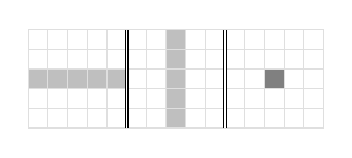
\begin{tikzpicture}[scale=0.25]
            \fill[gray!50]  (0 , 2) rectangle +(5, 1);
            \fill[gray!50]  (7 , 0) rectangle +(1, 5);
            \fill[gray!100] (12, 2) rectangle +(1, 1);
            \draw[step=1,gray!25] (0, 0) grid (15, 5);
            \draw[black, double] (5 , 0) -- +(0, 5);
            \draw[black, double] (10, 0) -- +(0, 5);
        \end{tikzpicture}
    }

    \caption{
        The access pattern for matrix multiplications on a single element \square{gray!100} that accesses \square{gray!50}.
    }
    \label{fig:matmult_access_pattern}
\end{figure}

Optimizing cache performance for matrix multiplications has been researched extensively.
Implementations either use a form of tiling, a divide and conquer strategy or different array structures to improve performance \cite{bader2006cache,frigo1999cache}.

The lower bound of matrix multiplication is not $O(n^3)$.
\citet{strassen1969gaussian}'s original algorithm and \citet{winograd1971multiplication}'s variation runs in $O(n^{2.81})$.
Note that the best bound is $\omega < 2.373$ for $O(n^\omega)$ \cite{alman2018limits}.
\citeauthor{strassen1969gaussian}'s algorithm has also been implemented on the GPU by \citet{li2011strassen}.

\section{Research Question}

% How much can we gain in accelerate
\begin{mdframed}
    \textbf{Research Question 1}
    \emph{What are the thread schedules for common structured GPGPU operations that result in the fastest execution?}
\end{mdframed}
A schedule optimal for one operation may not be optimal for another operation.
The optimal schedule is also dependent on the shape of the input data.
We are interested in the theoretical bounds of amounts of cache loads for a given schedule.
However, the scheduling can result in extra computation time, so we must also check with real world performance metrics.

% Comparison with current state of the art
\begin{mdframed}
    \textbf{Research Question 2}
    \emph{Is specialized structured scheduling equally or more performant than locality graph-based scheduling for structured GPGPU operations?}
\end{mdframed}
The PAVER method by \citet{tripathy2021paver} is the current state of the art regarding GPU scheduling.
We would like to see how well the proposed method compares to what is achievable.

\section{Approach}
The built-in GPU scheduler allocates threads and CTAs to streaming multiprocessors.
While the architecture does not guarantee an exact execution order of threads, it does group threads into CTAs deterministically and allocates these CTAs in a round-robin fashion.
We can therefore manipulate the scheduling by transforming the thread id.

The transformation can be implemented during the code generation phase in Accelerate, specifically by modifying the CUDA skeletons.
This allows us to manipulate the schedule depending on various (run-time) parameters such as input size, dimensionality, and GPU-architecture.

\subsection{Specialized Scheduling for Stencil Operations}
\label{sec:stencil_schedule}
Naive implementations of 2D stencil operations will go through the workload on a row-by-row basis.
However, if the input matrix is wide enough, data from the previous row can be unloaded before we can reuse it in the next row.
\citet{rivera2000tiling} suggest using tiling, including for higher dimension stencil operations however we propose an alternative method: \emph{column grouping}.
By splitting workload into fixed width columns we can keep as much data of the previous row(s) into cache as needed.
It would add an extra initial load when threads start working on new columns, but is negligible with sufficiently long columns.

In this case the size of cache correlates to the footprint of the stencil operation running on two rows of the column.
When working with multiple threads, an operation can start further ahead on the column.
We can estimate the size of the cache $M_{cache}$ with the stencil height $s_h$ and width $s_w$, column width $c_w$, number of threads $t$ and element size $e$:
\[
    M_{cache} = e (c_w + s_w) \left(s_h + \ceil{\frac{t}{c_w}}\right) 
\]
Given image height $I_h$, width $I_w$ and cache line width $M_{width}$, we can deduce the amount of cache misses.
The number of columns needed to cover the output is
\[
    \ceil{\frac{I_w}{c_w}}
\]
The number of rows needed
\[
    (s_h + I_h - 1)    
\]
Each row may span multiple cache lines. In the worst case, even if our row is smaller than $M_{width}$, it still may cross a cache line border
\[
    \ceil{\frac{s_w + c_w - 1}{M_{width}} + 1}
\]
Which can be combined to estimate the number of cache lines that needs to be brought into memory $M_{loads}$
\[
    M_{loads} = (s_h + I_h - 1)\ceil{\frac{s_w + c_w - 1}{M_{width}} + 1}\ceil{\frac{I_w}{c_w}}
\]

We want to minimize $M_{loads}$ by increasing the column width, while still staying within the $M_{cache}$ of our physical hardware.
There is also an incentive to keep $c_w$ to multiples of the cache line width to decrease the amount of cache line borders crossings.
The number of loads for various column configurations is compared to the best and worst case of the naive implementations in figure \ref{fig:matrix_loads}.

\begin{figure}
\centering
\subfloat[The $M_{loads}$ for a given $c_w$ that is a multiple of $M_{width}$. Naive describes the case where the cache is too small to share between stencil rows. Optimal describes the absolute minimum of loads possible, assuming the cache is large enough to fit the input array.]{
    \begin{tikzpicture}[>=stealth]
        \begin{axis}[
            width=0.45\textwidth,
            height=0.6\textwidth,
            cycle list/Dark2,
            mark=none,
            thick,
            xmode=log,
            ymode=log,
            log basis x=2,
            xtick={32, 64, 128, 256, 512},
            xlabel={$I_h\times I_w$},
            ylabel={$M_{loads}$},
            legend pos=north west,
            legend cell align={left},
            ]
            \addplot table [x=I, y=8,  col sep=comma] {loads_data/stencil_loads.csv};
            \addlegendentry{$C_w = 8$}
            
            %\addplot table [x=I, y= 16, col sep=comma] {loads_data/stencil_loads.csv};
            %\addlegendentry{$C_w = 16$}

            \addplot table [x=I, y=32, col sep=comma] {loads_data/stencil_loads.csv};
            \addlegendentry{$C_w = 32$}
            
            %\addplot table [x=I, y=64, col sep=comma] {loads_data/stencil_loads.csv};
            %\addlegendentry{$C_w = 64$}

            \addplot table [x=I, y=128, col sep=comma] {loads_data/stencil_loads.csv};
            \addlegendentry{$C_w = 128$}

            \addplot+[red] table [x=I, y=naive,  col sep=comma] {loads_data/stencil_loads.csv};
            \addlegendentry{Naive}

            \addplot+[black] table [x=I, y=naive_opt,  col sep=comma] {loads_data/stencil_loads.csv};
            \addlegendentry{Optimal}
        \end{axis}
    \end{tikzpicture}
}
\qquad
\subfloat[$c_w$ that are not a multiple of $M_{width}$ may perform better, but a multiple of $M_{width}$ may be preferred.]{
    \begin{tikzpicture}[>=stealth]
        \begin{axis}[
            width=0.45\textwidth,
            height=0.6\textwidth,
            cycle list/Dark2,
            mark=none,
            thick,
            xmin=100,
            xmax=300,
            xmode=log,
            ymode=log,
            log basis x=2,
            xtick={32, 64, 128, 256, 512},
            xlabel={$I_h\times I_w$},
            ylabel={$M_{loads}$},
            legend pos=north west,
            legend cell align={left},
            ]
            \addplot table [x=I, y=27, col sep=comma] {loads_data/stencil_loads.csv};
            \addlegendentry{$C_w = 27$}

            \addplot table [x=I, y=32, col sep=comma] {loads_data/stencil_loads.csv};
            \addlegendentry{$C_w = 32$}
            
            \addplot table [x=I, y=37, col sep=comma] {loads_data/stencil_loads.csv};
            \addlegendentry{$C_w = 37$}
        \end{axis}
    \end{tikzpicture}
}
\caption{
    The number of cache line load needed for a 7x7 stencil operation with various column widths $c_w$ for $M_{width} = 8$ and $s_h = s_w = 7$.
}
\label{fig:matrix_loads}
\end{figure}

\subsubsection{Preliminary Simulation}
\label{sec:stencil_sim}
We analyze the stencil pattern on a simulator with a simple LRU cache with the parameters in table \ref{tab:sim_stencil_params}. 
A time step consists out the calculation of a single element of the stencil in which we record the accessed addresses.
The state of each address at every time step is plot in a spatial-temporal diagram (fig. \ref{fig:st_stencil}) which can show us spatial and temporal locality.
Spatial locality can be identified by \square{black} vertical regions where accessed addresses can share the same cache line.
Temporal locality can be identified by \square{black} and \square{gray} horizontal regions where cached data stays in cache long enough to being reused. \square{red} regions are data that is brought into cache from memory, either due to being unloaded or being evicted earlier.

\begin{table}[H]
    \centering
    \begin{tabular}{|c c|}
        \hline
        Cache lines      & 24   \\
        Cache line width & 4    \\
        Eviction policy  & LRU  \\
        \hline
        Stencil size     & 7x7  \\
        Input Size       & 16x16\\
        Column size      & 8    \\
        \hline
    \end{tabular}
    \caption{
        The input parameters to generate figure \ref{fig:st_stencil}.
    }
    \label{tab:sim_stencil_params}
\end{table}

In the naive case we observe a large amount of cache misses (fig. \ref{fig:st_stencil_naive}).
This is because the cache is not large enough to allow for reuse when wrapping around to the next row of calculations.
The proposed method solves by also ensuring temporal locality (fig \ref{fig:st_stencil_column}).
The limited horizontal range from the columns can be observed in the zigzagging in the diagram.

\begin{figure}
    \centering
    \subfloat[The spatial temporal diagram of a 7x7 stencil with linear ordering.]{
        \begin{tikzpicture}
            \node (image) at (0,0) {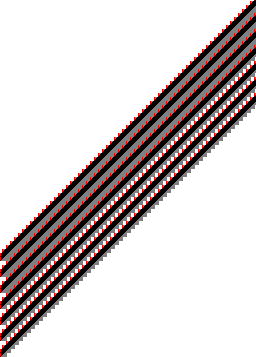
\includegraphics[width=0.4\textwidth]{st_diagrams/stencil7x7_linear.png}};
            \draw [->] (image.south west) -- ++(2,0) node[right]{\footnotesize\textit{Time}};
            \draw [->] (image.south west) -- ++(0,2) node[rotate=90, above]{\footnotesize\textit{Address}};
        \end{tikzpicture}
        \label{fig:st_stencil_naive}
    }
    \qquad
    \subfloat[The spatial temporal diagram of a 7x7 stencil with a column of size 4 ordering.]{
        \centering
        \begin{tikzpicture}
            \node (image) at (0,0) {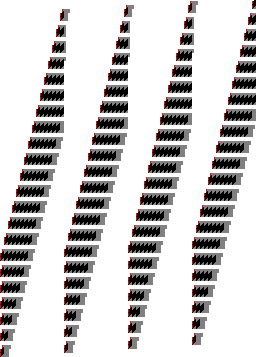
\includegraphics[width=0.4\textwidth]{st_diagrams/stencil7x7_column_4.png}};
            \draw [->] (image.south west) -- ++(2,0) node[right]{\footnotesize\textit{Time}};
            \draw [->] (image.south west) -- ++(0,2) node[rotate=90, above]{\footnotesize\textit{Address}};
        \end{tikzpicture}
        \label{fig:st_stencil_column}
    }

    \caption{
        The spatial temporal diagrams of a 7x7 stencil. The vertical axis describes the location in a 2D array which is mapped to 1D address space. The horizontal axis describes time. \square{red} are addresses of cache lines that are brought into cache. \square{black} are addresses being accessed. \square{gray} are addresses in cache.
    }
    \label{fig:st_stencil}
\end{figure}

\subsection{Specialized Scheduling for Matrix Multiplication}
\label{sec:matrix_schedule}
Let's look at improving cache performance on the naive $O(n^3)$ matrix multiplication.
In the ideal world, caches would be large enough to contain all the relevant matrices.
However, with inputs large enough we need to load data into cache multiple times.
A common optimization is to partition the work into tiles, however the column based method described in section \ref{sec:stencil_schedule} also works.

\subsubsection{Preliminary Simulation}

We run a similar simulation as in section \ref{sec:stencil_sim} with an adjusted amount of cache lines to account for the larger amount of memory processed (table \ref{tab:sim_matrix_params}).

\begin{table}[H]
    \centering
    \begin{tabular}{|c c|}
        \hline
        Cache lines      & 32   \\
        Cache line width & 4    \\
        Eviction policy  & LRU  \\
        \hline
        Input Size       & 16x16\\
        Column size      & 8    \\
        \hline
    \end{tabular}
    \caption{
        The input parameters to generate figure \ref{fig:st_matrix}.
    }
    \label{tab:sim_matrix_params}
\end{table}

The results are compiled into spatial temporal diagram (figure \ref{fig:st_matrix}).
With the original ordering, accessing the columns for each resulting element can lots of cache misses (figure \ref{fig:st_matrix_naive}).
The proposed schedule improves reuse by ensuring that columns in the same cache lines are reused as much as possible (figure \ref{fig:st_matrix_column}).
As a result we incur more cache misses on row accesses, but this is mitigated by the fact that these accesses are more efficient since more useful data is contained per cache line.

\begin{figure}
    \centering
    \subfloat[The spatial temporal diagram of a matrix multiplication with linear ordering.]{
        \begin{tikzpicture}[spy using outlines={rectangle, magnification=4,connect spies}]
            \node (image) at (0,0) {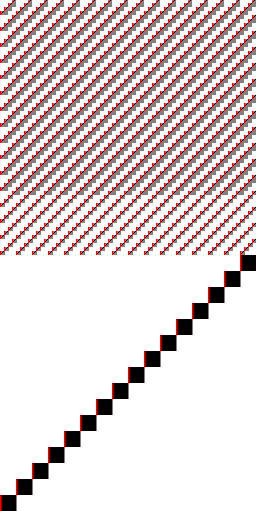
\includegraphics[width=0.25\textwidth]{st_diagrams/matrix_linear.png}};
            \draw [->] (image.south west) -- ++(2,0) node[right]{\footnotesize\textit{Time}};
            \draw [->] (image.south west) -- ++(0,8.5) node[rotate=90, above left]{\footnotesize\textit{Memory Addresses}};

            \coordinate (p) at (0, 1);
            \coordinate (v) at (3.3, 2);
            \spy[width=2.4cm,height=4cm] on (p) in node [fill=white] at (v);
        \end{tikzpicture}
        \label{fig:st_matrix_naive}
    }
    \qquad
    \subfloat[The spatial temporal diagram of a matrix multiplication with a column of size 4 ordering.]{
        \centering
        \begin{tikzpicture}[spy using outlines={rectangle, magnification=4,connect spies}]
            \node (image) at (0,0) {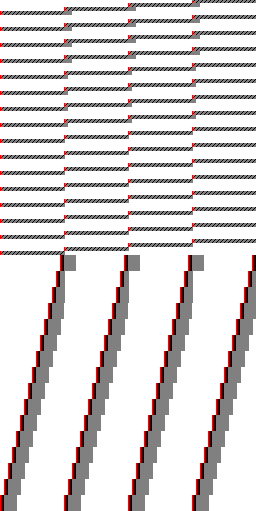
\includegraphics[width=0.25\textwidth]{st_diagrams/matrix_column_4.png}};
            \draw [->] (image.south west) -- ++(2,0) node[right]{\footnotesize\textit{Time}};
            \draw [->] (image.south west) -- ++(0,8.5) node[rotate=90, above left]{\footnotesize\textit{Memory Addresses}};

            \coordinate (p) at (0, 1);
            \coordinate (v) at (3.3, 2);
            \spy[width=2.4cm,height=4cm] on (p) in node [fill=white] at (v);
        \end{tikzpicture}
        \label{fig:st_matrix_column}
    }

    \caption{
        The spatial temporal diagrams of a matrix multiplication. The vertical axis describes the location in a 2D array which is mapped to 1D address space. The horizontal axis describes time. \square{red} are addresses of cache lines that are brought into cache. \square{black} are addresses being accessed. \square{gray} are addresses in cache.
    }
    \label{fig:st_matrix}
\end{figure}

There are, however, a matrix multiplication algorithms with a lower computation complexity. 
\citet{li2011strassen} has shown that it is possible to run Strassen's algorithm (discussed in section \ref{sec:matrix_intro}) on the GPU.
The implementation for a scheduler for Strassen's algorithm is lower priority and may or may not be implemented, since Accelerate does not have an implementation of it.

\subsection{Generate and Permute}

The permutation primitive initializes an array with default values and then combines it with the input array according to a combination function and an index map.
From a memory point of view we are interested in the predictable memory accesses which can be defined in terms of execution parameters per thread.
We categorize accesses as following:
\begin{itemize}
    \item \textbf{Horizontal} accesses that describe spatial locality. 
    While these can exploit cache lines the most, they may also cause inefficiencies by crossing cache line boundaries.
    
    \item \textbf{Vertical} accesses that describe temporal locality, due to any thread on the same column being able to reuse accessed data. From a memory perspective we simply have a fixed offset.
    
    \item \textbf{Streaming} accesses are only read once and are a prime target for cache bypassing, allowing other fused operations to use more cache.
    
    \item \textbf{Random} access are either values dependent on an earlier read value or both arbitrarily horizontal and vertical. While cache bypassing may prevent cache trashing when fused with another operator, it might reduce performance when accessing similar addresses.
\end{itemize}
Loading horizontally aligned data is much cheaper than loading vertically aligned data, since the latter may span multiple cache lines.
We therefore prioritize optimizing for vertical locality.
To exploit vertical locality, data must be kept in cache long enough.
For the column ordering described in section \ref{sec:stencil_schedule}, we can control how long data is stored in cache by increase or decrease $c_w$.
Having a generic method to determine $c_w$ allows us to incorporate fused operators since we only care about the relative offset and range of each memory access and the input of fused operators are thread indices.
\TODO{Incorporate citations}
\citet{balen2020optimal}
\citet{mcdonell2013optimising}

\subsection{Scan and Fold}
Scan primitives, also known as prefix sums, have many parallel algorithms.
However, due to the RAW relationship between threads there is less freedom to tweak the scheduling.
Fold primitives are similar to scan primitives, but instead only return a single element.
The same (or partial) strategies used in scan can be used for folds.
Due to both primitives having high data dependency between threads and there being multiple algorithms, we will not look at the scan and fold primitives unless time allows.

\subsection{Planning}
The idea is to first work on simpler discrete problems to get familiar with Accelerate and setting a baseline of improvements.
Then generalize the scheduler to work for any structured schedule where threads may work independently of each other.
The planning is as following:
\begin{itemize}
    \item \textbf{Week 1:} Stencil scheduler implementation.
    \item \textbf{Week 2:} Stencil benchmarks.
    \item \textbf{Week 3:} Matrix multiplication scheduler implementation.
    \item \textbf{Week 4:} Matrix benchmarks.
    \item \textbf{Week 5, 6:} Analysis for required column width for any structured program.
    \item \textbf{Week 7, 8:} Implementation of analysis.
    \item \textbf{Week 9:} Scheduler implementation for any structured program.
    \item \textbf{Week 10, 11, 12:} PAVER implementation.
    \item \textbf{Week 12, 13, 14:} Paper writing.
    \item \textbf{Week 15, 16:} Reserved for delays or further improvements.
\end{itemize}

\subsection{Preliminary Results}
To test the viability of thread scheduling, zigzagging has been implemented for stencil operations.
For a 9x9 box averaging stencil on a 4k matrix it resulted in a 13\% decrease from 2.08ms to 1.79ms in kernel run times on a RTX 2080 Super.


%\end{multicols}

\bibliographystyle{unsrtnat}
\bibliography{bibliography}
\end{document}
